\providecommand{\topdir}{..}
\documentclass[../main.tex]{subfiles}


\begin{document}
	\chapter{Resonant X-ray Electric Field Intensity}\label{chap:07-res-XEFI}
	\section{Experimental Setup}

	\begin{figure}[H]
		\centering
		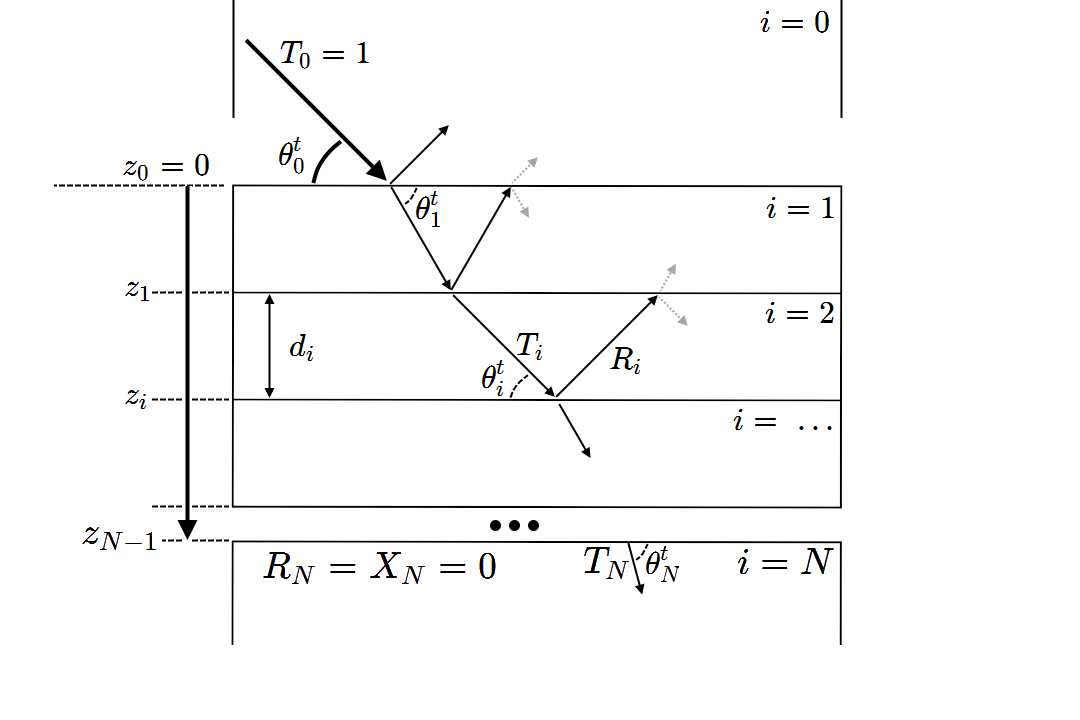
\includegraphics[width=0.8\textwidth]{resources/ch7/geometry.png}
		\caption{Experimental setup for measuring the X-ray electric field intensity. The X-ray beam is incident on a sample, and the reflected beam is analyzed to determine the electric field intensity. Here there are N+1 layers, including the first layer (i.e. vacuum/air) and the substrate both of which are semi-infinite. The interfaces are indexed between two layers $i$ and $i+1$, such that interface is positioned at $z_i$. This same indexing is used for any interface calculations, such as the Fresnel coefficients.}
		\label{fig:experimental-setup}
	\end{figure}

	\subsection{Electric field}
	The total electric field of the X-ray beam in any given layer is given by the summation of two propogating waves.
	\begin{align}
		\vec{E_i}(\vec{r}) &= \vec{T_i}(\vec{r}) + \vec{R_i}(\vec{r})
	\end{align}
	where 
	\begin{align}
		\vec{T_i}(\vec{r}) &= T_i \cdot \exp\left(-\mathbf{i} \vec{k_{i}} \cdot \vec{r}\right) \\
		\vec{R_i}(\vec{r}) &= R_i \cdot \exp\left(+\mathbf{i} \vec{k_{i}} \cdot \vec{r}\right)
	\end{align}
	and $\vec{k_i}$ is the wavevector of the X-ray beam in layer $i$, at position $\vec{r}$.
	
	Here the transmission and reflection components represent the sum of all multiple-scattering events in the layer.
	The complex constants $T_i$ and $R_i$ result of the requirement for continuity of the electric field vector at the boundary - more specifically, through a recursive solution using the Fresnel coefficients for each interface.

	Typically, especially for non-resonant X-ray scattering, the x-component wavevector $k_x$ is ignored and the attenuation is treated as negligible.

	\subsection{Angle of incidence and wavevector}
	For any radiation of wavelength $\lambda$, and incident angle $\theta_0$ coming from vacuum or a medium of complex refractive index $N$,
	the corresponding wavevector $\vec{k}$ is given by
	\begin{align}
		\vec{k_0} = \frac{2 \pi}{\lambda} \left( \cos(\theta_0) \hat{x} + \sin(\theta_0) \hat{z} \right)
	\end{align}
	
	As the X-ray propogates through the sample, the dielectric constant modifies the (now complex) angle of incidence and the complex wavevector, as per Snell's law (for grazing incidence).

	% TODO: Fix up equation for K_i....
	\begin{align}
		\theta_i &= \arccos\left(\frac{\cos\left(\theta_0\right) \times N_0}{N_i}\right)\\
		\vec{k_i} &= \left( |k_{0}|\cos\theta_0 \hat{x} + |k_0| \sqrt{n_i^2 - \cos^2\theta_i} \hat{z} \right)
	\end{align}	

	Notice here that the attenuation of the X-ray beam in the x-direction has a constant wavevector component that is real


	\subsubsection{Critical angle}
	For any given refractive index $N_i < N_0$ \footnote{This is usually the case for X-rays where $N_i = 1 - \delta_i + \mathbf{i}\beta_i$}, the critical angle occurs when $\cos\left(\theta_0\right) < \frac{N_i}{N_0}$.
	In the case where $N_0 \approxeq 1$ is air/vacuum, this critical angle corresponds to
	\begin{align}
		\theta_{0} &= \sqrt{2 \delta_i}
	\end{align}

	\section{Interface Calculation}
	To calculate the effect of refraction and reflection at each interface, a boundary condition is applied that the tangential component of the electric field must be continuous across the interface (both in $\hat{x}$ and $\hat{y}$ directions). This requires knowledge of the polarisation of the X-ray beam, as well as the refractive index of the medium.

	For convention, we define positive $\hat{z}$ out of the film; $z$ is negative as it penetrates into the film. $\hat{x}$ is positive along the beam path, and monotonically increases. As the x-ray propogates some space in the film (i.e., -ve z and +ve x), the phase contribution is $\exp\left[\mathbf{i}\vec{k}\cdot\vec{r}\right]$.
	Hence the sign of the wavevector components also match the direction of the beam: negative $k_z$ and positive $k_x$, such that the imaginary component of the wavevector leads to a decaying wave in the film.

	\subsection{Polarisation Dependence}
	An x-ray can be S-polarised (parallel to the planar surface, i.e. in the $\hat{y}$ or $\hat{x}$ direction) or P-polarised (parallel to the planar normal, i.e. in the $\hat{z}$ plane). These are also known as transverse electric (TE) and transverse magnetic (TM) polarisations, respectively.

	Usually, the polarisation angle $\alpha$ can be defined as the angle between the electric field vector and the plane of incidence, with $\alpha = 0$ for S-polarised waves and $\alpha = \frac{\pi}{2}$ for P-polarised waves. Then the perpendicular and parallel components of the electric field vector can be defined as
	\begin{align}
		E_{i, \perp} &= E_i \cos(\alpha) \\
		E_{i, \parallel} &= E_i \sin(\alpha)
	\end{align}

	In the context of grazing incidence experiments, the X-ray beam is typically highly aligned and polarised. It will be routine to perform measurements with both S- and P-polarised X-rays.

	\subsection{Fresnel Coefficients}
	Fresnel coefficients describe the amplitude of reflected and transmitted waves at an interface between two media with different refractive indices. For S-polarised waves, the Fresnel coefficients are given by
	\begin{align}
		t_{i, i+1}^{s} &= \frac{2 k_{i, z}}{k_{i, z} + k_{i+1, z}} \\
		r_{i, i+1}^{s} &= \frac{k_{i, z} - k_{i+1, z}}{k_{i,z} + k_{i+1,z}} = t_{s,i} - 1
	\end{align}
	For P-polarised waves, the Fresnel coefficients are given by
	\begin{align}
		t_{i, i+1}^{p} &= \frac{2 k_{i, z}}{n^2 k_{i, z} + k_{i+1, z}} \\
		r_{i, i+1}^{p} &= \frac{n^2 k_{i+1, z} - k_{i, z}}{n^2 k_{i+1,z} + k_{i,z}}
	\end{align}
	At resonance, the refractive index $n$ can be modified by a significant amount. Consider the imaginary component in Polystyrene (CH) at the carbon K edge changing magnitude from 1e-4 to 6e-3. For P3MEEET (C\textsubscript{11}H\textsubscript{16}O\textsubscript{3}S) at the resonant sulfur K edge, the magnitude changes from 9e-7 to 5.7e-6.

	The polarisation dependence for the Fresnel coefficients is not significantly changed by $n^2$, so we approximate using the s-polarisation case.

	\section{Taylor series result for the reflected electric field between multiple interfaces}
	Following the derivation of Borne \& Wolf (1985) and Savakhin et al. (2020), we derive the electric field in a multi-layer system, accounting for decaying x-propogation of waves.

	In any layer, the total electric field is the sum of many reflections.
	\begin{align}
		E_j = E_{j,1} + E_{j,2} + E_{j,3} + ... + E_{j,N} + ...
	\end{align}
	
	Considering an interface with a transmitted wave $E^t_{j}$ into layer $j$ and the corresponding total incident wave $E_{j-1}$ from the previous layer.
	\begin{align}
		E_{j,1} &= E^t_{j} \exp\left[\mathbf{i}\left(\vec{k_j}\cdot \vec{r}\right)\right] \\
		&= E_{j-1} t_{j-1,j} \exp\left[\mathbf{i}\left(\vec{k_j}\cdot \vec{r}\right)\right] \\
		&= E_{j-1} 
			\left(1 + r_{j-1,j}\right)
			\exp\left[\mathbf{i}\left(\vec{k_j}\cdot \vec{r}\right)\right]
	\end{align}
	
	Secondly, we follow a reflection from the bottom interface between layers $j,j+1$, with reflection coefficient $r_{j,j+1}$. The wave has now travelled additional vertical distance between the two interfaces, so we relabel the z-components $d_{j}$ for the thickness between interfaces $z_i$ and $z_{i+1}$. 
	
	\vspace{1em}
	\textbf{This section is incorrect - it forgets that the x-component wavevector is constant due to boundary conditions hahahaha. Such are the mistakes of trying new things.}
	\vspace{1em}

	Importantly, and deviating from previous results, we also track the horizontal distance travelled in terms of $d_{j}$, as $\tan(\theta_j) = d_{j} / c_{j}$, where $\theta_j$ is the angle of incidence in layer $j$ between interfaces $i, i+1$. While this distance is continuously increasing (i.e. there's no phase subtraction), we need to observe the decay of the wave is propogates forwards. We therefore write $x \to \delta x$, where $\delta x < c_{j}$. Considering only the z position abstracts decaying reflections, and therefore leads to incorrect results.

	\begin{align}
		E_{j,2} &=\begin{aligned}[t]
				&E_{j-1}	
				\left(1 + r_{j-1,j}\right) \times r_{j, j+1} \\
				&\exp\left[\mathbf{i}\left((2 d_{j} - z) k_{j,z} + x k_{j,x}  \right)\right]
			\end{aligned} \\
			&=\begin{aligned}[t]
				&E_{j-1} 
				\left(1 + r_{j-1,j}\right) \times r_{j, j+1}\\
				&\exp\left[\mathbf{i}\left((2 d_{j} - z) k_{j,z}\right)\right]
				\exp\left[\mathbf{i}\left((c_{j} + \delta x) k_{j,x}\right)\right]
			\end{aligned}
	\end{align}

	The third component is a surface reflection from the top interface, noting that $r_{j,j-1} = -r_{j-1,j}$, corresponding to a phase shift of $\pi$.
	\begin{align}
		E_{j,3} &= 
			\begin{aligned}[t]
			&E_{j-1} 
			\left(1 + r_{j-1,j}\right) \times r_{j, j+1} \times (- r_{j-1,j})\\
			&\exp\left[\mathbf{i}\left((2 d_{j} + z) k_{j,z}\right)\right]
			\exp\left[\mathbf{i}\left((2 c_{j} + \delta x) k_{j,x}\right)\right]
			\end{aligned}
	\end{align}

	The fourth component is another surface reflection from the bottom surface.
	\begin{align}
		E_{j,4} &= 
			\begin{aligned}[t]
			&E_{j-1} 
			\left(1 + r_{j-1,j}\right) \times r_{j, j+1} \times (- r_{j-1,j}) \times (r_{j, j+1})\\
			&\exp\left[\mathbf{i}\left((4 d_{j} - z) k_{j,z}\right)\right]
			\exp\left[\mathbf{i}\left((3 c_{j} + \delta x) k_{j,x}\right)\right]
			\end{aligned}\\
			&= 
			\begin{aligned}[t]
			&E_{j-1} 
			\left(1 + r_{j-1,j}\right) \times r_{j, j+1}^2 \times (- r_{j-1,j})\\
			&\exp\left[\mathbf{i}\left((4 d_{j} - z) k_{j,z}\right)\right]
			\exp\left[\mathbf{i}\left((3 c_{j} + \delta x) k_{j,x}\right)\right]
			\end{aligned}
	\end{align}

	The fifth component is another surface reflection from the top surface.
	\begin{align}
		E_{j,5} &= 
			\begin{aligned}[t]
			&E_{j-1} 
			\left(1 + r_{j-1,j}\right) \times r_{j, j+1}^2 \times (-r_{j-1,j})^2\\
			&\exp\left[\mathbf{i}\left((4 d_{j} + z) k_{j,z}\right)\right]
			\exp\left[\mathbf{i}\left((4 c_{j} + \delta x) k_{j,x}\right)\right]
			\end{aligned}
	\end{align}
	And so on. Considering the remaining $\delta x$ as a function of z, we can parametrise this as:
	\begin{align}
		\delta x = \left\{
			\begin{aligned}
			(z){\tan\theta_j}^{-1} && N &\in 2\mathds{Z} + 1 &&\text{ (odd)}\\
			(d-z){\tan\theta_j}^{-1} && N &\in 2\mathds{Z} &&\text{ (even)}
		\end{aligned}
		\right.
	\end{align}
	This leads to the following sets of expressions for forward and backward propogating waves corresponding to odd and even $N$.
	\begin{align}
		E_{j,N} &= E_{j-1} \left(1 + r_{j-1,j}\right) \times
			 \left\{ \begin{aligned}
			&\begin{aligned}[c]
			& r_{j, j+1}^{(N-1)/2} \times (-r_{j-1,j})^{(N-1)/2}\\
			&\times \exp\left[\mathbf{i}k_{j,z}\left((N-1) d_{j} + z\right) \right]\\
			&\times \exp\left[\mathbf{i}k_{j,x}\left(\left(N-1\right) c_{j} + z{\tan\theta_j}^{-1}\right) \right]
			\end{aligned}
			&&& N &\in 2\mathds{Z} + 1 &&\text{ (odd)}\\
			\\
			&\begin{aligned}[c]
			& r_{j, j+1}^{N/2} \times (-r_{j-1,j})^{N/2-1}\\
			& \times\exp\left[\mathbf{i}k_{j,z}\left(N d_{j} - z\right) \right]\\
			& \times\exp\left[\mathbf{i}k_{j,x}\left((N-1) c_{j} + (d_j-z){\tan\theta_j}^{-1}\right) \right]
			\end{aligned}
			&&& N &\in 2\mathds{Z} &&\text{ (even)}
		\end{aligned}\right.
	\end{align}

	Also note $\left((N-1) c_{j} + (d_j-z){\tan\theta_j}^{-1}\right) \equiv Nc_j - z{\tan\theta_j}^{-1}$, simplifying the even expression.

	The total sum of all reflections can then be written as a geometric series where the common component of the odd/even terms is factored in $\zeta$:
	\begin{align}
		E_j &= 
		\begin{aligned}[t]
			&E_{j-1}(1+r_{j-1,j}) \times \zeta \\
			&\times \left(
			\begin{aligned}[c]
				&\exp\left[\mathbf{i}\left( k_{j,z} + k_{j,x}{\tan\theta_j}^{-1}\right)z\right]\\
				+ r_{j, j+1} 
				&\exp\left[\mathbf{i}\left( k_{j,z} + k_{j,x}{\tan\theta_j}^{-1}\right)\left(2d_j - z\right)\right]
			\end{aligned}
			\right)
		\end{aligned}\\
		\zeta &= \begin{aligned}[t]
			1 &- r_{j-1,j}r_{j,j+1}\exp\left[\mathbf{i}(2(k_{j,z} + k_{j,x}{\tan\theta_j}^{-1}) d_j)\right] \\
			&+ r_{j-1,j}^2r_{j,j+1}^2\exp\left[\mathbf{i}(4(k_{j,z} + k_{j,x}{\tan\theta_j}^{-1}) d_j)\right]\\
			&- ...
		\end{aligned}
	\end{align}

	We recognise the Taylor expansion form of $1/(1+x)$, with the expression for $x$ being $x=r_{j-1,j}r_{j,j+1}\exp\left[\mathbf{i}(2(k_{j,z} + k_{j,x}{\tan\theta_j}^{-1}) d_j)\right]$. Thus the series can be written as:
	\begin{align}
		E_j &= \begin{aligned}[t]
			&E_{j-1}\left(1 + r_{j-1,j}\right)\\
			&\times
			\dfrac{
					\exp\left[-\mathbf{i}(k_{j,z} + k_{j,x}{\tan\theta_j}^{-1}) z\right]
					+ 	r_{j,j+1} 
						\exp\left[\mathbf{i}(k_{j,z} + k_{j,x}{\tan\theta_j}^{-1})(2d_j - z)\right]
				}
				{1 + r_{j-1,j}r_{j,j+1}
				\exp\left[\mathbf{i}(2 (k_{j,z} + k_{j,x}{\tan\theta_j}^{-1}) d_j)\right]
				}
		\end{aligned}
	\end{align}

	\subsection{Separating the reflection and transmission summation coefficients similar to Dev et al. (2020) and }

	


	\ifSubfilesClassLoaded{
		\printbibliography{}
		\printglossaries
	}{} % we have no 'else' action
	
\end{document}